% Options for packages loaded elsewhere
\PassOptionsToPackage{unicode}{hyperref}
\PassOptionsToPackage{hyphens}{url}
%
\documentclass[
]{book}
\usepackage{amsmath,amssymb}
\usepackage{lmodern}
\usepackage{ifxetex,ifluatex}
\ifnum 0\ifxetex 1\fi\ifluatex 1\fi=0 % if pdftex
  \usepackage[T1]{fontenc}
  \usepackage[utf8]{inputenc}
  \usepackage{textcomp} % provide euro and other symbols
\else % if luatex or xetex
  \usepackage{unicode-math}
  \defaultfontfeatures{Scale=MatchLowercase}
  \defaultfontfeatures[\rmfamily]{Ligatures=TeX,Scale=1}
\fi
% Use upquote if available, for straight quotes in verbatim environments
\IfFileExists{upquote.sty}{\usepackage{upquote}}{}
\IfFileExists{microtype.sty}{% use microtype if available
  \usepackage[]{microtype}
  \UseMicrotypeSet[protrusion]{basicmath} % disable protrusion for tt fonts
}{}
\makeatletter
\@ifundefined{KOMAClassName}{% if non-KOMA class
  \IfFileExists{parskip.sty}{%
    \usepackage{parskip}
  }{% else
    \setlength{\parindent}{0pt}
    \setlength{\parskip}{6pt plus 2pt minus 1pt}}
}{% if KOMA class
  \KOMAoptions{parskip=half}}
\makeatother
\usepackage{xcolor}
\IfFileExists{xurl.sty}{\usepackage{xurl}}{} % add URL line breaks if available
\IfFileExists{bookmark.sty}{\usepackage{bookmark}}{\usepackage{hyperref}}
\hypersetup{
  pdftitle={SPI-IPM Code Manual},
  pdfauthor={Chloé R. Nater},
  hidelinks,
  pdfcreator={LaTeX via pandoc}}
\urlstyle{same} % disable monospaced font for URLs
\usepackage{longtable,booktabs,array}
\usepackage{calc} % for calculating minipage widths
% Correct order of tables after \paragraph or \subparagraph
\usepackage{etoolbox}
\makeatletter
\patchcmd\longtable{\par}{\if@noskipsec\mbox{}\fi\par}{}{}
\makeatother
% Allow footnotes in longtable head/foot
\IfFileExists{footnotehyper.sty}{\usepackage{footnotehyper}}{\usepackage{footnote}}
\makesavenoteenv{longtable}
\usepackage{graphicx}
\makeatletter
\def\maxwidth{\ifdim\Gin@nat@width>\linewidth\linewidth\else\Gin@nat@width\fi}
\def\maxheight{\ifdim\Gin@nat@height>\textheight\textheight\else\Gin@nat@height\fi}
\makeatother
% Scale images if necessary, so that they will not overflow the page
% margins by default, and it is still possible to overwrite the defaults
% using explicit options in \includegraphics[width, height, ...]{}
\setkeys{Gin}{width=\maxwidth,height=\maxheight,keepaspectratio}
% Set default figure placement to htbp
\makeatletter
\def\fps@figure{htbp}
\makeatother
\setlength{\emergencystretch}{3em} % prevent overfull lines
\providecommand{\tightlist}{%
  \setlength{\itemsep}{0pt}\setlength{\parskip}{0pt}}
\setcounter{secnumdepth}{5}
\usepackage{booktabs}
\usepackage{amsthm}
\makeatletter
\def\thm@space@setup{%
  \thm@preskip=8pt plus 2pt minus 4pt
  \thm@postskip=\thm@preskip
}
\makeatother
\ifluatex
  \usepackage{selnolig}  % disable illegal ligatures
\fi
\usepackage[]{natbib}
\bibliographystyle{apalike}

\title{SPI-IPM Code Manual}
\author{Chloé R. Nater}
\date{2021-08-19}

\begin{document}
\maketitle

{
\setcounter{tocdepth}{1}
\tableofcontents
}
\hypertarget{about-this-manual}{%
\chapter*{About this manual}\label{about-this-manual}}
\addcontentsline{toc}{chapter}{About this manual}

Briefly on the need for/value of standardized data and analyses.

Why IPMs are popular and what they are suitable for \citep{kery2011, plard2019}.

Overview over workflow, code repository \& contents of manual (Figure \ref{fig:WorkflowDiag}).

\begin{figure}

{\centering 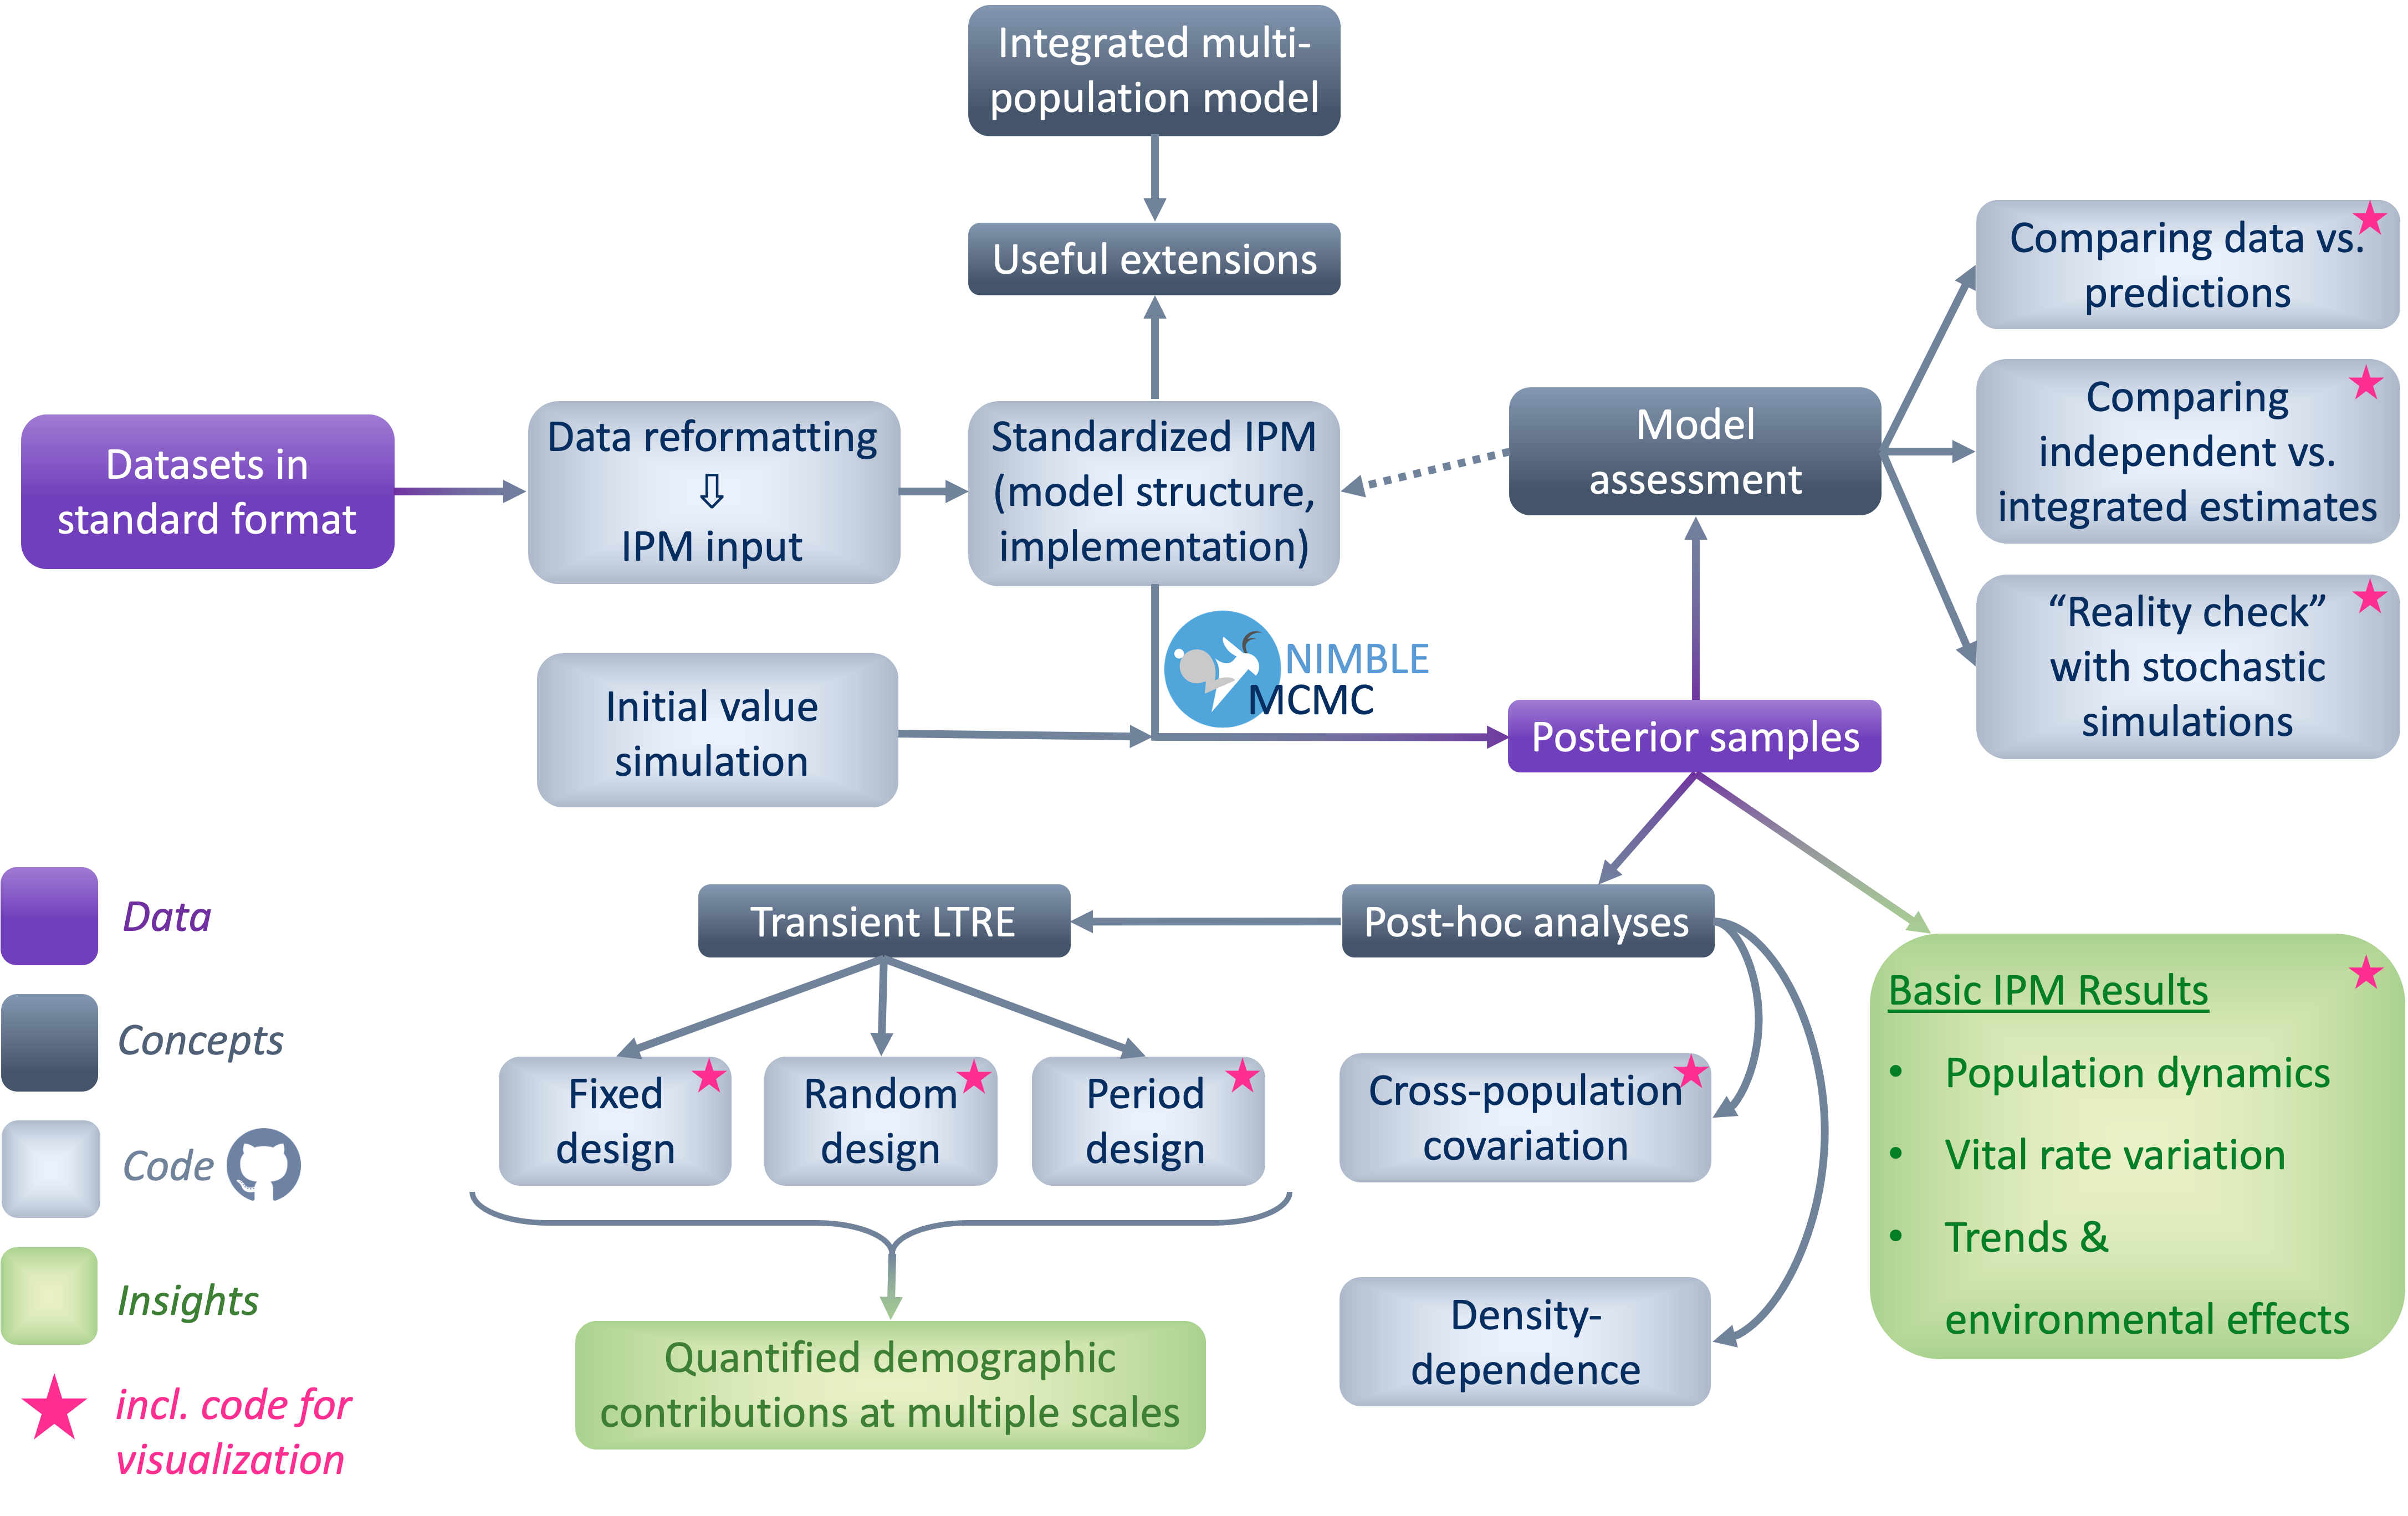
\includegraphics[width=1\linewidth]{Figures/SPI-IPM_Workflow} 

}

\caption{Schematic representation of the SPI-IPM workflow.}\label{fig:WorkflowDiag}
\end{figure}

In no way complete: great if user's analyses/adaptations become part.

How to cite.

\hypertarget{DataPrep}{%
\chapter{Preparing SPI-Birds data for Bayesian analysis}\label{DataPrep}}

Quick recap of SPI-Birds standard format and overview over data types used in IPM (+ how they relate, incl.~diagram).

\hypertarget{nest-count-data}{%
\section{Nest count data}\label{nest-count-data}}

\hypertarget{clutch-size-data}{%
\section{Clutch size data}\label{clutch-size-data}}

\hypertarget{nest-level}{%
\subsection{Nest level}\label{nest-level}}

\hypertarget{population-level}{%
\subsection{Population level}\label{population-level}}

\hypertarget{fledgling-count-data}{%
\section{Fledgling count data}\label{fledgling-count-data}}

\hypertarget{nest-level-1}{%
\subsection{Nest level}\label{nest-level-1}}

\hypertarget{population-level-1}{%
\subsection{Population level}\label{population-level-1}}

\hypertarget{mark-recapture-data}{%
\section{Mark-recapture data}\label{mark-recapture-data}}

\hypertarget{individual-capture-histories}{%
\subsection{Individual capture histories}\label{individual-capture-histories}}

\hypertarget{m-array}{%
\subsection{M-array}\label{m-array}}

\hypertarget{immigrant-count-data}{%
\section{Immigrant count data}\label{immigrant-count-data}}

\hypertarget{auxiliary-data-on-the-sampling-process}{%
\section{Auxiliary data on the sampling process}\label{auxiliary-data-on-the-sampling-process}}

\hypertarget{nest-survey-sampling-effort}{%
\subsection{Nest survey sampling effort}\label{nest-survey-sampling-effort}}

\hypertarget{capture-probability-proxies}{%
\subsection{Capture probability proxies}\label{capture-probability-proxies}}

\hypertarget{IPMCon}{%
\chapter{IPM Construction}\label{IPMCon}}

\hypertarget{open-population-model-with-2-age-classes}{%
\section{Open population model with 2 age classes}\label{open-population-model-with-2-age-classes}}

\hypertarget{data-likelihoods}{%
\section{Data likelihoods}\label{data-likelihoods}}

\hypertarget{nest-count-data-likelihood}{%
\subsection{Nest count data likelihood}\label{nest-count-data-likelihood}}

\hypertarget{clutch-size-data-likelihoods}{%
\subsection{Clutch size data likelihoods}\label{clutch-size-data-likelihoods}}

\hypertarget{fledgling-count-data-likelihoods}{%
\subsection{Fledgling count data likelihoods}\label{fledgling-count-data-likelihoods}}

\hypertarget{mark-recapture-data-likelihood}{%
\subsection{Mark-recapture data likelihood}\label{mark-recapture-data-likelihood}}

\hypertarget{immigrant-count-data-likelihood}{%
\subsection{Immigrant count data likelihood}\label{immigrant-count-data-likelihood}}

\hypertarget{priors-and-constraints}{%
\section{Priors and constraints}\label{priors-and-constraints}}

\hypertarget{TempVar}{%
\chapter{Modelling temporal variation}\label{TempVar}}

\hypertarget{random-year-variation}{%
\section{Random year variation}\label{random-year-variation}}

\hypertarget{temporal-covariates}{%
\section{Temporal covariates}\label{temporal-covariates}}

\hypertarget{continuous-variables}{%
\subsection{Continuous variables}\label{continuous-variables}}

\hypertarget{categorical-variables}{%
\subsection{Categorical variables}\label{categorical-variables}}

\hypertarget{imputation-of-missing-covariate-values}{%
\subsection{Imputation of missing covariate values}\label{imputation-of-missing-covariate-values}}

\hypertarget{notes-on-covariate-selection}{%
\section{Notes on covariate selection}\label{notes-on-covariate-selection}}

\hypertarget{IPMImp}{%
\chapter{IPM Implementation}\label{IPMImp}}

\hypertarget{efficient-implementation-using-nimble}{%
\section{Efficient implementation using NIMBLE}\label{efficient-implementation-using-nimble}}

We use the fantastic \textbf{nimble} package \citep{devalpine2017}!

\hypertarget{simulation-of-initial-values}{%
\section{Simulation of initial values}\label{simulation-of-initial-values}}

\hypertarget{test-runs-and-full-runs-chains-iterations-burn-in-and-thinning}{%
\section{Test runs and full runs: chains, iterations, burn-in, and thinning}\label{test-runs-and-full-runs-chains-iterations-burn-in-and-thinning}}

\hypertarget{trouble-shooting-implementation-issues}{%
\section{Trouble-shooting implementation issues}\label{trouble-shooting-implementation-issues}}

\hypertarget{ModelAssm}{%
\chapter{Model Assessment}\label{ModelAssm}}

\hypertarget{assessing-chain-convergence}{%
\section{Assessing chain convergence}\label{assessing-chain-convergence}}

\hypertarget{plotting-data-vs.-predictions}{%
\section{Plotting data vs.~predictions}\label{plotting-data-vs.-predictions}}

\hypertarget{comparing-estimates-from-integrated-vs.-independent-analyses}{%
\section{Comparing estimates from integrated vs.~independent analyses}\label{comparing-estimates-from-integrated-vs.-independent-analyses}}

\hypertarget{reality-check-using-stochastic-simulations}{%
\section{``Reality check'' using stochastic simulations}\label{reality-check-using-stochastic-simulations}}

\hypertarget{other-approaches}{%
\section{Other approaches}\label{other-approaches}}

Running for additional years and comparing to non-included data, PPCs, etc.

\hypertarget{ResultsViz}{%
\chapter{Visualizing and interpreting direct IPM outputs}\label{ResultsViz}}

\hypertarget{population-trajectories}{%
\section{Population trajectories}\label{population-trajectories}}

\hypertarget{within-population-variation-in-vital-rates}{%
\section{Within-population variation in vital rates}\label{within-population-variation-in-vital-rates}}

\hypertarget{age-class-specific-averages}{%
\subsection{Age-class-specific averages}\label{age-class-specific-averages}}

\hypertarget{year-by-year-variation}{%
\subsection{Year-by-year variation}\label{year-by-year-variation}}

\hypertarget{between-population-variation-in-vital-rates}{%
\section{Between-population variation in vital rates}\label{between-population-variation-in-vital-rates}}

\hypertarget{population-specific-averages}{%
\subsection{Population-specific averages}\label{population-specific-averages}}

\hypertarget{year-by-year-variation-1}{%
\subsection{Year-by-year variation}\label{year-by-year-variation-1}}

\hypertarget{covariate-effects}{%
\section{Covariate effects}\label{covariate-effects}}

\hypertarget{AddAnalyses}{%
\chapter{Follow-up Analyses}\label{AddAnalyses}}

\hypertarget{testing-for-time-trends}{%
\section{Testing for time-trends}\label{testing-for-time-trends}}

\hypertarget{testing-for-density-dependence}{%
\section{Testing for density-dependence}\label{testing-for-density-dependence}}

\hypertarget{investigating-cross-population-covariation}{%
\section{Investigating cross-population covariation}\label{investigating-cross-population-covariation}}

\hypertarget{quantifying-demographic-contributions-to-short-term-population-dynamics}{%
\section{Quantifying demographic contributions to short term population dynamics}\label{quantifying-demographic-contributions-to-short-term-population-dynamics}}

\hypertarget{year-by-year-variation-in-population-growth-rate-random-design-ltre}{%
\subsection{Year-by-year variation in population growth rate (random design LTRE)}\label{year-by-year-variation-in-population-growth-rate-random-design-ltre}}

\hypertarget{year-to-year-differences-in-population-growth-rate-fixed-design-ltre}{%
\subsection{Year-to-year differences in population growth rate (fixed design LTRE)}\label{year-to-year-differences-in-population-growth-rate-fixed-design-ltre}}

\hypertarget{quantifying-demographic-contributions-to-long-term-population-trends}{%
\section{Quantifying demographic contributions to long-term population trends}\label{quantifying-demographic-contributions-to-long-term-population-trends}}

\hypertarget{differences-in-population-trajectories-between-time-periods-period-design-ltre}{%
\subsection{Differences in population trajectories between time periods (period design LTRE)}\label{differences-in-population-trajectories-between-time-periods-period-design-ltre}}

\hypertarget{differences-in-population-trajectories-between-locations-period-design-ltre-with-time-by-space-substitution}{%
\subsection{Differences in population trajectories between locations (period design LTRE with time-by-space substitution)}\label{differences-in-population-trajectories-between-locations-period-design-ltre-with-time-by-space-substitution}}

\hypertarget{ExtOutlook}{%
\chapter{Useful extensions and outlook}\label{ExtOutlook}}

\hypertarget{adapting-the-population-model-for-your-speciespopulation}{%
\section{Adapting the population model for your species/population}\label{adapting-the-population-model-for-your-speciespopulation}}

\hypertarget{accounting-for-multiple-broods-per-bird-per-year}{%
\subsection{Accounting for multiple broods per bird per year}\label{accounting-for-multiple-broods-per-bird-per-year}}

\hypertarget{altering-age-structure}{%
\subsection{Altering age structure}\label{altering-age-structure}}

\hypertarget{individual-heterogeneity-beyond-age-sex-traits-and-more}{%
\subsection{Individual heterogeneity beyond age: sex, traits, and more}\label{individual-heterogeneity-beyond-age-sex-traits-and-more}}

\hypertarget{including-additional-data-and-informative-priors}{%
\section{Including additional data and informative priors}\label{including-additional-data-and-informative-priors}}

\hypertarget{including-partially-observed-age-information}{%
\subsection{Including partially observed age information}\label{including-partially-observed-age-information}}

\hypertarget{making-the-most-of-auxiliary-knowledge-about-immigrantsdispersers}{%
\subsection{Making the most of auxiliary knowledge about immigrants/dispersers}\label{making-the-most-of-auxiliary-knowledge-about-immigrantsdispersers}}

\hypertarget{letting-published-values-help-with-estimation-when-data-is-sparse}{%
\subsection{Letting published values help with estimation when data is sparse}\label{letting-published-values-help-with-estimation-when-data-is-sparse}}

\hypertarget{building-on-the-multi-population-perspective}{%
\section{Building on the multi-population perspective}\label{building-on-the-multi-population-perspective}}

\hypertarget{joint-analysis-of-data-from-several-populations}{%
\subsection{Joint analysis of data from several populations}\label{joint-analysis-of-data-from-several-populations}}

\hypertarget{modelling-cross-population-covariation}{%
\subsection{Modelling cross-population covariation}\label{modelling-cross-population-covariation}}

\hypertarget{estimating-hyper-parameters-in-large-scale-analyses}{%
\subsection{Estimating hyper-parameters in large-scale analyses}\label{estimating-hyper-parameters-in-large-scale-analyses}}

\hypertarget{unlocking-the-secrets-of-dispersal}{%
\subsection{Unlocking the secrets of dispersal}\label{unlocking-the-secrets-of-dispersal}}

  \bibliography{book.bib,packages.bib}

\end{document}
